\documentclass[12pt]{article}
\usepackage[utf8]{inputenc}
\usepackage{geometry, setspace}
\geometry{a4paper, portrait, margin=1in}
\usepackage{amsmath}
\usepackage{graphicx}
\usepackage{float}
\usepackage{minted}
\usepackage{hyperref}
\usepackage{setspace}
\usepackage{caption, subcaption}
\usepackage[title]{appendix}
\usepackage{booktabs, tabularx}
\usepackage{tikz}
% \usepackage{indentfirst}
\hypersetup{
    colorlinks,
    citecolor=black,
    filecolor=black,
    linkcolor=black,
    urlcolor=black
}

\newtheorem{definition}{Definition}
\newtheorem{lemma}{Lemma}

\begin{document}
% --------- title page -------------
\begin{titlepage}
    \begin{center}
        \vspace*{1cm}
 
        \LARGE\textbf{Near-Optimal Schedule Rendering by Graph Coloring}
   
        \vspace{1.5cm}
 
        \textbf{Hanzhi Zhou}
 
        \vfill
        \vspace{0.8cm}

        \Large
        School of Engineering and Applied Science\\
        \vspace{0.2cm}
        University of Virginia\\
        \vspace{0.2cm}
        \today
        \vspace{1cm}
    \end{center}
    \clearpage
\end{titlepage}

\section{Introduction}

\section{Graph Representation}
\begin{figure}[H]
    \centering
    \begin{subfigure}{.4\textwidth}
        \centering
        \includegraphics[width=.8\columnwidth]{example1}
        \caption{A Simple Schedule}
        \label{fig:exp1}
    \end{subfigure}%
    \begin{subfigure}{.6\textwidth}
        \centering
        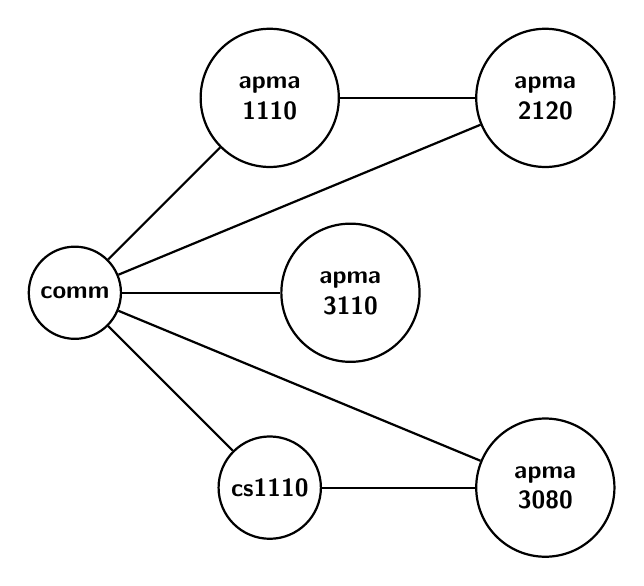
\begin{tikzpicture}[auto, node distance=3.5cm, every loop/.style={},
            thick,main node/.style={circle,draw,font=\sffamily\bfseries\small}]
        
        \node[main node] (comm) {comm};
        \node[main node] (apma1110) [above right of=comm] {\begin{tabular}{c}
            apma \\ 1110
        \end{tabular}};
        \node[main node] (apma2120) [right of=apma1110] {\begin{tabular}{c}
            apma \\ 2120
        \end{tabular}};
        \node[main node] (apma3110) [right of=comm] {\begin{tabular}{c}
            apma \\ 3110
        \end{tabular}};
        \node[main node] (cs1110) [below right of=comm] {cs1110};
        \node[main node] (apma3080) [right of=cs1110] {\begin{tabular}{c}
            apma \\ 3080
        \end{tabular}};

        \path[every node/.style={font=\sffamily\small}]
        (comm) edge node { } (apma1110)
        (comm) edge node { } (apma2120)
        (comm) edge node { } (apma3110)
        (comm) edge node { } (apma3080)
        (apma1110) edge node { } (apma2120)
        (cs1110) edge node { } (apma3080)
        (comm) edge node { } (cs1110);
        \end{tikzpicture}
        \caption{Graph Representation}
        \label{fig:graphexp1}
    \end{subfigure}%
    \caption{}
    \label{}
\end{figure}

\begin{definition}
    Two events are said to be \textbf{conflicting} iff the time periods in which they take place have overlap.
\end{definition}

\begin{definition}
    Slots are positions in a column that contain events. They are uniquely identified by their \textbf{left}.
\end{definition}

\begin{lemma}
    The \textbf{time period}, \textbf{width} and \textbf{left} of an event are sufficient to render an event
\end{lemma}

The main principle behind schedule rendering is that two conflicting events cannot have the same left, otherwise there must be a part where they appear to overlap with one another.
The k-colorability problem asks whether it is possible to color the vertices of a graph using k colors, subject to the condition that no two adjacent nodes have the same color. We can slightly modify the problem statement so its applicable to our problem: given a set of events, some of which may have conflicts, is it possible to allocate k \textbf{slots} such that no two adjacent (conflicting) events occupy the same \textbf{slot}.

From our new problem statement, we arrive at the graph representation of the set of events that we want to render.

\begin{definition}\label{def:3}
    Each event is represented as a \textbf{node (vertex)}, and every two nodes are connected by an edge iff they have conflict.
\end{definition}

Using definition~\ref{def:3}, we can construct a graph for the set of events shown in Figure~\ref{fig:exp1}. The resulting graph is shown in Figure~\ref{fig:graphexp1}.

\section{DFS Approach}

\end{document}